\documentclass[12pt]{article}

	\usepackage{answers}
	\usepackage{float}
	\usepackage{setspace}
	\usepackage{graphicx}
	\usepackage{enumitem}
	\usepackage{multicol}
	\usepackage{mathrsfs}
	\usepackage{listings}
	\usepackage[margin=1in]{geometry} 
	\usepackage{amsmath,amsthm,amssymb}
	 
	\usepackage[margin=0cm]{caption}
	 
	\newcommand{\N}{\mathbb{N}}
	\newcommand{\Z}{\mathbb{Z}}
	\newcommand{\C}{\mathbb{C}}
	\newcommand{\R}{\mathbb{R}}
	
	\DeclareMathOperator{\sech}{sech}
	\DeclareMathOperator{\csch}{csch}
	 
	\newenvironment{theorem}[2][Theorem]{\begin{trivlist}
	\item[\hskip \labelsep {\bfseries #1}\hskip \labelsep {\bfseries #2.}]}{\end{trivlist}}
	\newenvironment{definition}[2][Definition]{\begin{trivlist}
	\item[\hskip \labelsep {\bfseries #1}\hskip \labelsep {\bfseries #2.}]}{\end{trivlist}}
	\newenvironment{proposition}[2][Proposition]{\begin{trivlist}
	\item[\hskip \labelsep {\bfseries #1}\hskip \labelsep {\bfseries #2.}]}{\end{trivlist}}
	\newenvironment{lemma}[2][Lemma]{\begin{trivlist}
	\item[\hskip \labelsep {\bfseries #1}\hskip \labelsep {\bfseries #2.}]}{\end{trivlist}}
	\newenvironment{exercise}[2][Exercise]{\begin{trivlist}
	\item[\hskip \labelsep {\bfseries #1}\hskip \labelsep {\bfseries #2.}]}{\end{trivlist}}
	\newenvironment{solution}[2][Solution]{\begin{trivlist}
	\item[\hskip \labelsep {\bfseries #1}]}{\end{trivlist}}
	\newenvironment{problem}[2][Problem]{\begin{trivlist}
	\item[\hskip \labelsep {\bfseries #1}\hskip \labelsep {\bfseries #2.}]}{\end{trivlist}}
	\newenvironment{question}[2][Question]{\begin{trivlist}
	\item[\hskip \labelsep {\bfseries #1}\hskip \labelsep {\bfseries #2.}]}{\end{trivlist}}
	\newenvironment{corollary}[2][Corollary]{\begin{trivlist}
	\item[\hskip \labelsep {\bfseries #1}\hskip \labelsep {\bfseries #2.}]}{\end{trivlist}}
	 
	\begin{document}
	 
	% --------------------------------------------------------------
	%                         Start here
	% --------------------------------------------------------------
	 
	\title{Homework 2}%replace with the appropriate homework number
	\author{Christian Steinmetz\\ %replace with your name
	MATH 8090-Spring 2018} %if necessary, replace with your course title
	 
	\maketitle
	
	\begin{problem}{6}
	$ $ \\
	By matching the autocovariances and sample autocovariances at lags 0 and 1,
	fit a model of the form
	\begin{equation*}
		X_t - \mu = \phi(X_{t-1} - \mu) + Z_t,  \quad \{{Z_t}\} \sim WN(0, \sigma^2)
	\end{equation*}
	to the data STRIKES.TSM of Example 1.1.6. Use the fitted model to compute
	the best predictor of the number of strikes in 1981. Estimate the mean squared
	error of your predictor and construct 95\% prediction bounds for the number of
	strikes in 1981 assuming that
	\begin{equation*}
	\{{Z_t}\} \sim \text{iid} \ N(0, \sigma^2)
	\end{equation*}
	
	\end{problem}
	
	\begin{solution}{}
		
	\end{solution}
	\pagebreak
	
	\begin{problem}{7}
	$ $
	\begin{enumerate}[label=(\alph*)]
		\item Fit a linear regression using ols (lm function in R) and plot the ACF and PACF of the residuals. Are these plots consistent with an AR(1) model?
		\item Fit a linear trend with AR(1) errors to the global temperature data. use the predict function to predict the next two observations. Show how R is using the coefficients and data to calculate the predictions and use (3.3.19) to verify the calculation of the standard errors for the predictions. 
	\end{enumerate}
	\end{problem}
		
	\begin{solution}{}
	$ $
	\begin{enumerate}[label=(\alph*)]
		\item 
		
		\begin{figure}[H]
    			\centering
    			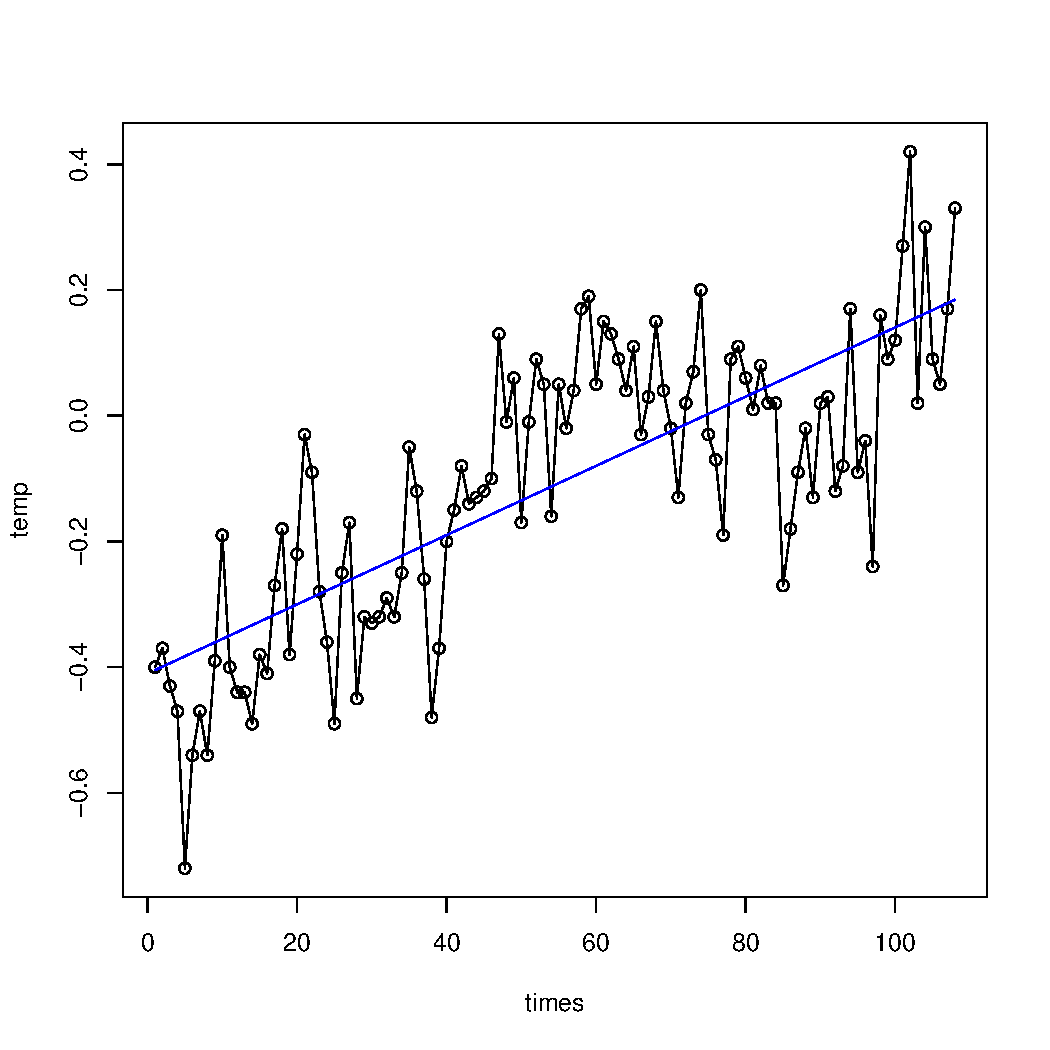
\includegraphics[width=0.6\textwidth]{figs/problem_7/temp_ols.pdf}
    			\caption{Linear regression trend using ols fitted to global temperature data.}
    			\label{fig:monthly_model}
		\end{figure}
		
		\begin{figure}[H]
    			\centering
    			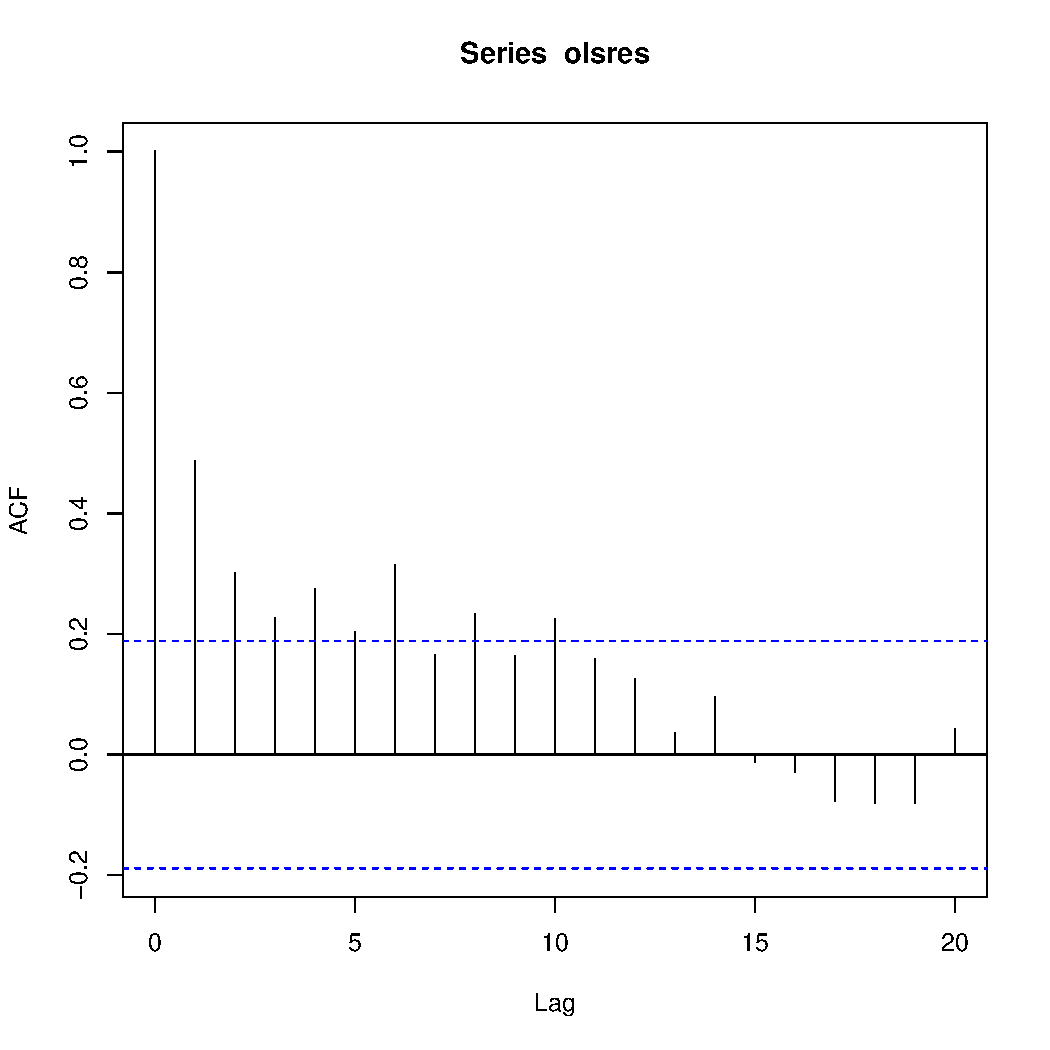
\includegraphics[width=0.6\textwidth]{figs/problem_7/temp_acf.pdf}
    			\caption{ACF of residuals from linear regression fit.}
    			\label{fig:monthly_model}
		\end{figure}

		\begin{figure}[H]
    			\centering
    			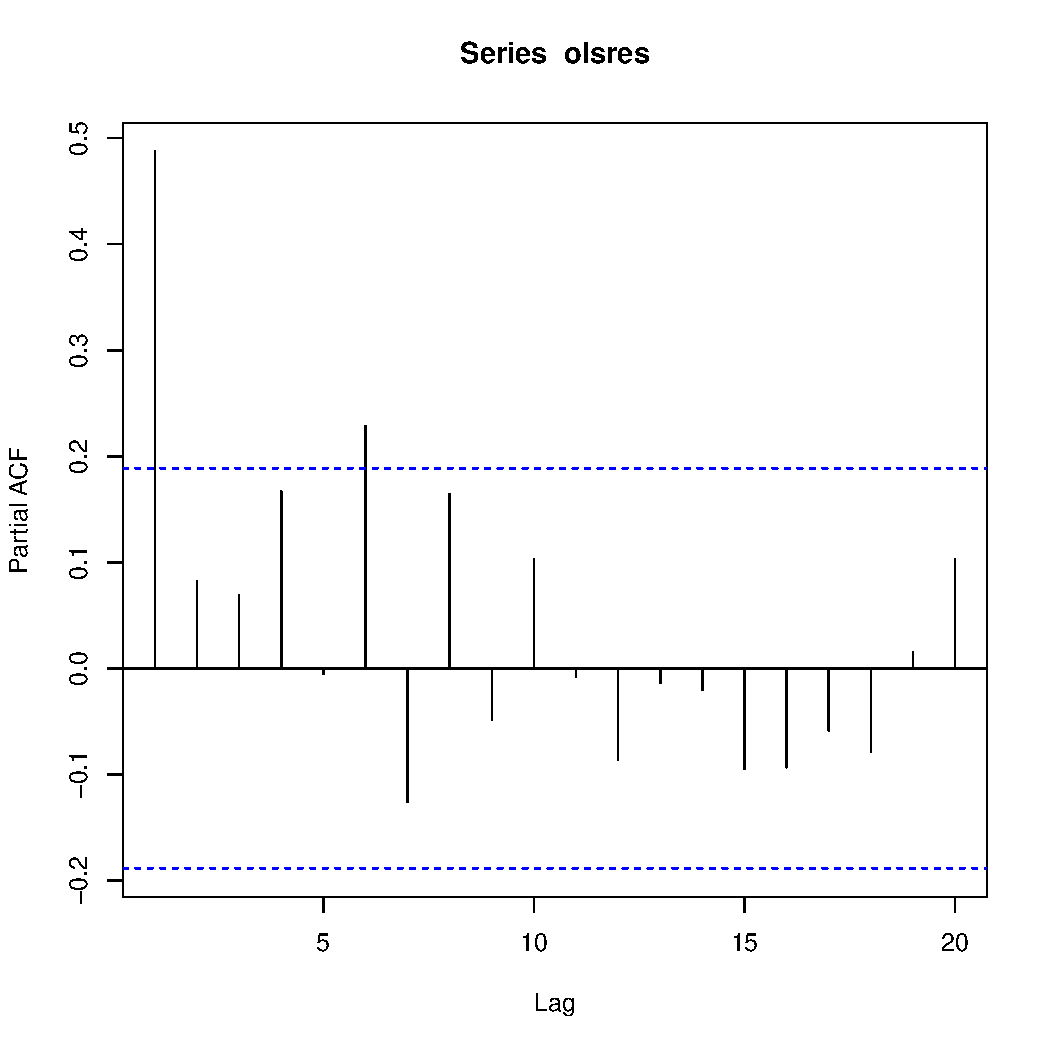
\includegraphics[width=0.6\textwidth]{figs/problem_7/temp_pacf.pdf}
    			\caption{PACF of residuals from linear regression fit.}
    			\label{fig:monthly_model}
		\end{figure}

		\item 
		
		\begin{figure}[H]
    			\centering
    			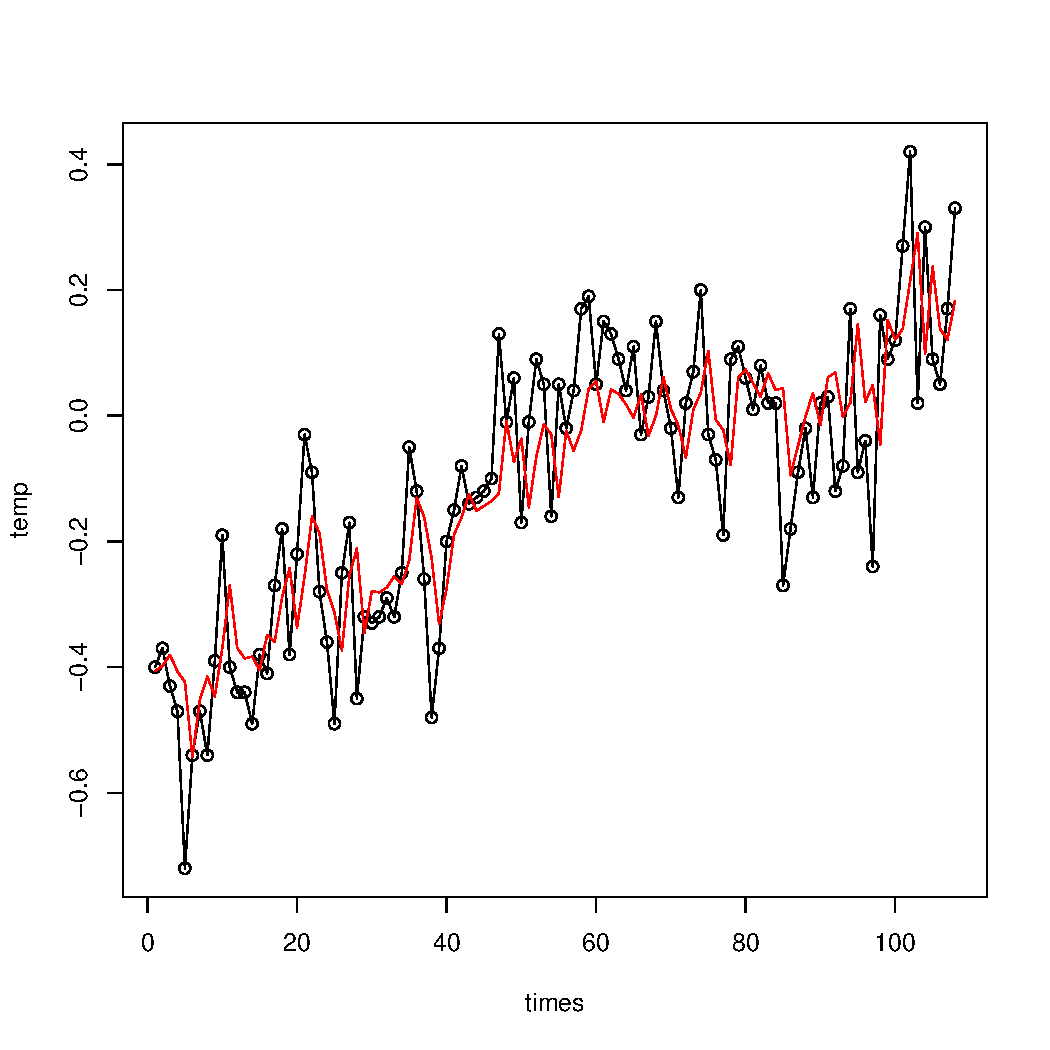
\includegraphics[width=0.6\textwidth]{figs/problem_7/temp_ar1_lin.pdf}
    			\caption{Linear trend with AR(1) fitted to the global temperature data..}
    			\label{fig:monthly_model}
		\end{figure}

		
	\end{enumerate}
	\end{solution}
	\pagebreak
	
	\end{document}
	